\textbf{4-1.}地球的质量是月球的 81 倍。地球和月球的中心相距 $3.84 \times 10^{8} \mathrm{~m}$ , 求地球和月球组成的系统的质心与地球中心的距离。

\begin{figure}[H]
  \centering
  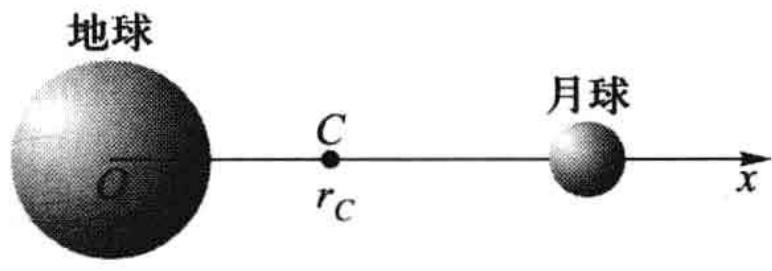
\includegraphics[width=0.4\textwidth]{figures/fig4-1.jpg}
  \end{figure}

\vfill

\textbf{4-2.}$A 、 B 、 C$ 三质点在某一时刻的位置坐标分别为: $(-3, 4, 3)$ 、 $(3, -8, 6)$ 、 $(1, 2, -1)$ , 坐标以 $\mathrm{m}$ 为单位, $B$ 的质量是 $A$ 的两倍, 而 $C$ 的质量是 $A$ 的三倍。求此时由此三质点组成的体系的质心的位置。

\vfill
\newpage

\textbf{4-3.}长为 $l$ 、线密度为 $\rho_{l}$ 的柔软绳索, 原先两端点 $A 、 B$ 并合一起, 悬挂在支点上, 现让 $B$ 端脱离支点自由下落, 求当 $B$ 端下落了 $x$ 时, 支点上所受的力 $F_{\mathrm{T}}$ 。

\begin{figure}[H]
  \centering
  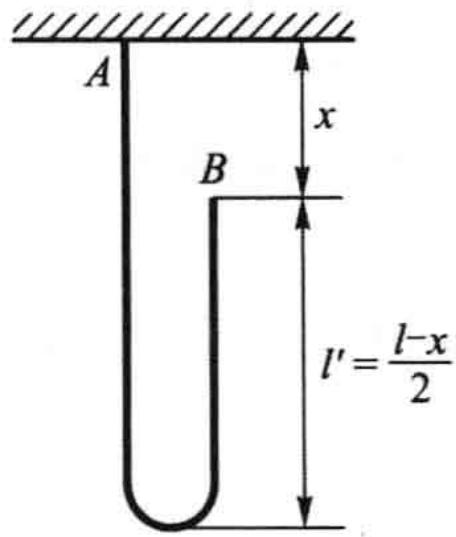
\includegraphics[width=0.2\textwidth]{figures/fig4-3.jpg}
  \end{figure}

\vfill

\textbf{4-4.}如习题 4-4 图所示, 光滑水平面上并排静放着两块质量分别为 $m_{1}$ 和

$m_{2}$ 的木块。一质量为 m 的子弹以初速度 $v_{0}$ 水平射向两木块，射穿两木块后以 $v'$ 的速度沿原方向运动。求两木块的速度 $v_{1}$ 和 $v_{2}$ 。设子弹在两木块中受到的阻力（可视为恒力）相等，而穿过 $m_{1}$ 所用的时间为穿过 $m_{2}$ 所用时间的一半。

\begin{figure}[H]
  \centering
  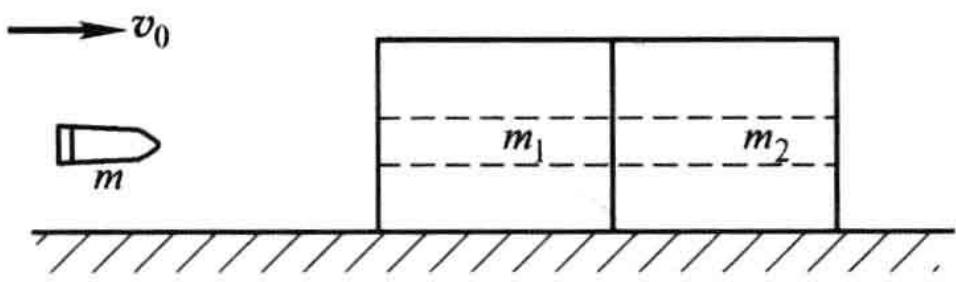
\includegraphics[width=0.4\textwidth]{figures/fig4-4.jpg}
  \end{figure}

\vfill
\newpage

\textbf{4-5.}一块长为 $L$ 的大平板静放在光滑水平冰面上, 一小孩骑着儿童自行车以 $v_{0}$ 的速度从板的一端驶上平板, 在板上他的速度忽快忽慢, 在将近板的另一端时, 他相对板的速度为 $u$ 。此时, 他忽然刹车, 在板的另一端边缘车相对板静止。已知人在板上骑车的时间为 $t$ , 板的质量为 $m_{0}$ , 小孩与车一起的质量为 $m$ 。试求:

(1) 刹车前瞬时板的速度;

(2) 车相对板刚静止时板的位移。

\vfill

\textbf{4-6.}两个质量分别为 $m_{1}$ 和 $m_{2} (m_{1} > m_{2})$ 的人身高相同, 他们同时以相同的速率竖直上跳, 在空中二人用力互推。若胖人的落地点距起跳点为 $s$ , 则瘦人的落地点距起跳点多远?

\vfill
\newpage

\textbf{4-7.}质量为 $m_{0}$ , 长为 $l$ 的小船静浮于河中, 小船两头分别站着质量为 $m_{1}$ 和

$m_{2}(m_{1}>m_{2})$ 的人,他们同时相对船以相同的速率 u 走向原位于船正中,但固定在河中的木桩,如习题 4-7 图所示。若忽略水对船的阻力作用,试问:

(1) 谁先走到木桩处?

(2) 他用了多少时间？

\begin{figure}[H]
  \centering
  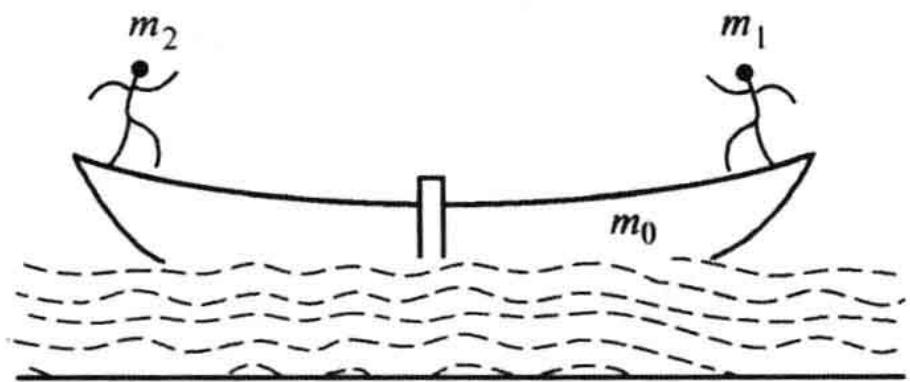
\includegraphics[width=0.3\textwidth]{figures/fig4-7.jpg}
  \end{figure}

\vfill

\textbf{4-8.}一质量为 $m_{1}$ 的杂技演员, 从蹦床上沿竖直方向跳起。当他上升到某一高度时, 迅速抱起边上栖木上的质量为 $m_{2}$ 的猴子, 结果他又上升了相同的高度然后落下。试求此种情况下杂技演员所能上升的高度 $h$ 与他不抱猴子所能达到的最大高度 $h_{0}$ 之比。

\vfill
\newpage

\textbf{4-9.}一火箭竖直向上发射, 当它达到最高点时炸裂成三个等质量的碎片, 观察到其中一块碎片经时间 $t_1$ 竖直地落到地上, 而其他两块碎片在炸裂后的 $t_2$ 时刻落在地上, 求火箭炸裂时离地面的高度。

\vfill

\textbf{4-10.}将一空盒放在秤盘上,并将秤的读数调整到零,然后从高出盒底 $h$ 处将小钢珠以每秒 $B$ 个的速率由静止开始掉入盒内,每一小钢珠的质量为 $m$ 。若钢珠与盒底碰撞后即静止,忽略小球在空中的时间,试求自钢珠落入盒内起,经过时间 $t$ 后秤的读数。

\vfill
\newpage

\textbf{4-11.}由喷泉中喷出的水柱, 把一个质量为 $m$ 的垃圾桶倒顶在空中。水以恒定的速率 $v_{0}$ 从面积为 $S$ 的小孔中喷出, 射向空中, 在冲击垃圾桶桶底以后, 有一半的水吸附在桶底, 并顺内壁流下, 其速度可忽略, 而另一半则以原速竖直溅下。求垃圾桶停留的高度 $h$ 。

\vfill

\textbf{4-12.}一质量为 $m_{0}$ (无水时) 的水桶开始时处于静止状态, 桶中装有质量为 $m$ 的水, 通过一根绳子施以恒力 $F$ 将桶从井中提上来, 桶中的水以恒定的质量速率从桶中漏出来, 经过时间 $t$ 桶变成空的。求变成空桶的瞬间桶的速度。

\vfill
\newpage

\textbf{4-13.}求均质的内外半径分别为 $a$ 和 $b$ 的半球壳的质心。

\vfill

\textbf{4-14.}在光滑的水平面上有两个质量分别为 $m_{1}$ 和 $m_{2}$ 的物体。它们中间用

一根原长为 l，劲度系数为 k 的弹簧相连，如习题 4-14 图所示。开始时，将 $m_{1}$ 紧靠墙，并将弹簧压缩至原长的 $\frac{1}{2}$ ，然后将 $m_{2}$ 释放。若以 $m_{1}$ 、 $m_{2}$ 和弹簧为系统，试求：

(1) 系统质心的加速度随时间的变化关系;

(2) 系统质心的速度最大值。

\begin{figure}[H]
  \centering
  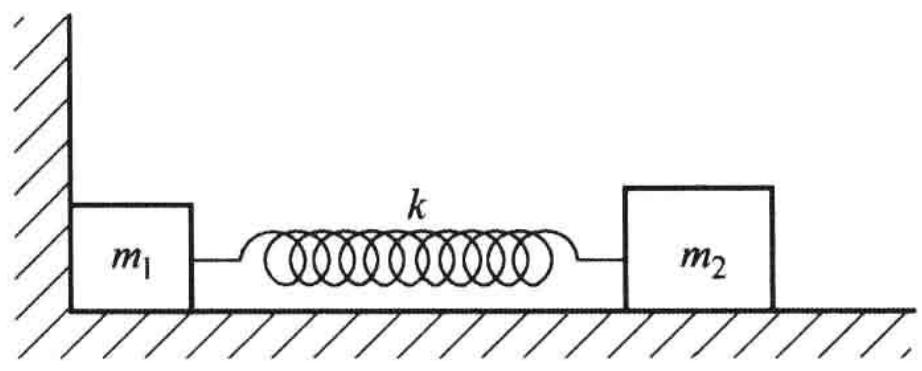
\includegraphics[width=0.4\textwidth]{figures/fig4-14_1.jpg}
  \end{figure}

\vfill
\newpage

\textbf{4-15.}一圆锥摆的摆线长为 $l$ , 摆锤的质量为 $m$ , 圆锥的半顶角为 $\alpha$ 。试求当摆锤从习题 4-15 图中位置 $A$ 沿圆周匀速运动到位置 $B$ 的过程中张力的冲量。

\begin{figure}[H]
  \centering
  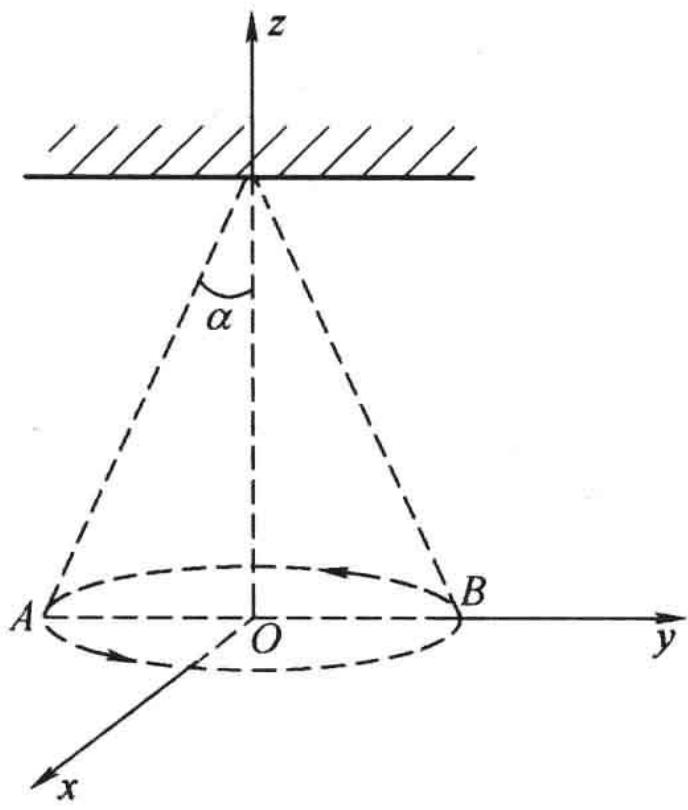
\includegraphics[width=0.3\textwidth]{figures/fig4-15.jpg}
  \end{figure}

\vfill

\textbf{4-16.}两质量皆为 $m_0$ 的冰车头尾相接地静止在光滑的水平冰面上。一质量为 $m$ 的人从一车跳到另一车, 然后再跳回。试证明: 两冰车的末速度之比为 $\frac{m_0 + m}{m_0}$ 。

\vfill
\newpage

\textbf{4-17.}如习题 4-17 图所示, 质量为 $m$ 的物体从静止下落 $y$ 后开始拉起质量为 $m_{0}(m_{0}>m)$ 的物体。两物体通过一根很轻且不可伸长的细绳相连并挂在一固定的光滑滑轮上。(1) 求物体 $m_{0}$ 返回原来位置所用的时间; (2) 求物体 $m_{0}$ 被拉起运动时系统减少的动能与原动能的比值。

\begin{figure}[H]
  \centering
  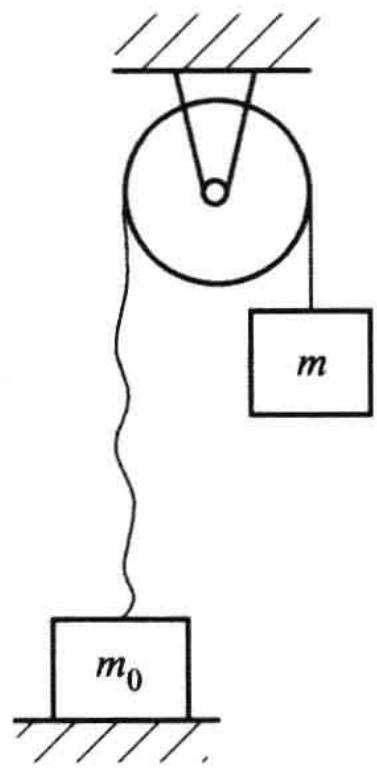
\includegraphics[width=0.18\textwidth]{figures/fig4-17.jpg}
  \end{figure}

\vfill

\textbf{4-18.}质量为 $m_{0}$ 的人手里拿着一个质量为 $m$ 的物体, 以 $v_{0}$ 的初速度向与地平线成 $\alpha$ 角的方向跳去, 当他达到最高点时, 将物体以相对速度 $u$ 水平向后抛出。问由于物体的抛出, 人向前跳出的距离增加了多少?

\vfill
\newpage

\textbf{4-19.}一质量为 $m$ 的男孩站在质量为 $m_0$ 的雪橇上以恒定的速度 $v_i$ 在冰面上滑行。若男孩沿与 $v_i$ 相反的方向在雪橇上跑动, 在离开雪橇末端时相对于雪橇的速率为 v。求雪橇相对于冰面的末速度。

\vfill

\textbf{4-20.}有 $N$ 个人站在铁路上静止的质量为 $m_0$ 的平板车上, 每人的质量均为 $m$ 。他们以相对于平板车的速度 $u$ 跳离平板车。设平板车与轨道间无摩擦力。

(1) 若所有的人同时跳,则平板车的最终速度是多少?

(2) 若他们一个一个地跳, 则平板车的最终速度是多少?

(3) 以上两种情况中哪一种的最终速度大些?

\vfill
\newpage

\textbf{4-21.}一质量 $m_{1} = 50 \mathrm{~kg}$ 的人 A 手里拿着一质量 $m = 5.0 \mathrm{~kg}$ 的小球以 $v_{1} = 1.2 \mathrm{~m} / \mathrm{s}$ 的速率在光滑冰面上沿直线滑冰, 而另一质量 $m_{2} = 45 \mathrm{~kg}$ 的人 B 以 $v_{2} = 0.8 \mathrm{~m} / \mathrm{s}$ 的速率向 A 对面滑来, 为避免碰撞, A 把球以相对于他的速率 $u$ 向 B 水平抛去, 让 B 接住。试问 $u$ 至少应多大?

\vfill

\textbf{4-22.}质量为 $m_{\mathrm{A}}$ 与 $m_{\mathrm{B}}$ 的两个小球 $\mathrm{A}$ 和 $\mathrm{B}$ , 用不可伸长的轻绳相连, 静止在水平面上。绳子拉紧时, 给 $\mathrm{B}$ 球一个冲量 $\mathbf{I}$ ,

I 的方向与 AB 连线成 $\alpha$ 角, $\alpha < \frac{\pi}{2}$ , 如习题 4-22 图所示。已知冲击后的速度 $v_{B}$ 的大小, 求 $v_{B}$ 的方向和冲量 I 的大小。

\begin{figure}[H]
  \centering
  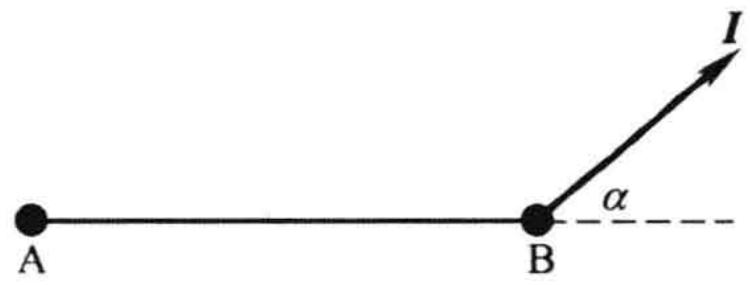
\includegraphics[width=0.4\textwidth]{figures/fig4-22.jpg}
  \end{figure}

\vfill
\newpage

\textbf{4-23.}如习题 4-23 图所示, 漏斗中的煤粉不断地落到速度 $v = 1.5 \mathrm{~m} / \mathrm{s}$ 的自动传送带上, 每秒钟落下的煤粉量为 $20 \mathrm{~kg}$ 。求煤粉作用在传送带上的水平方向的力。

\begin{figure}[H]
  \centering
  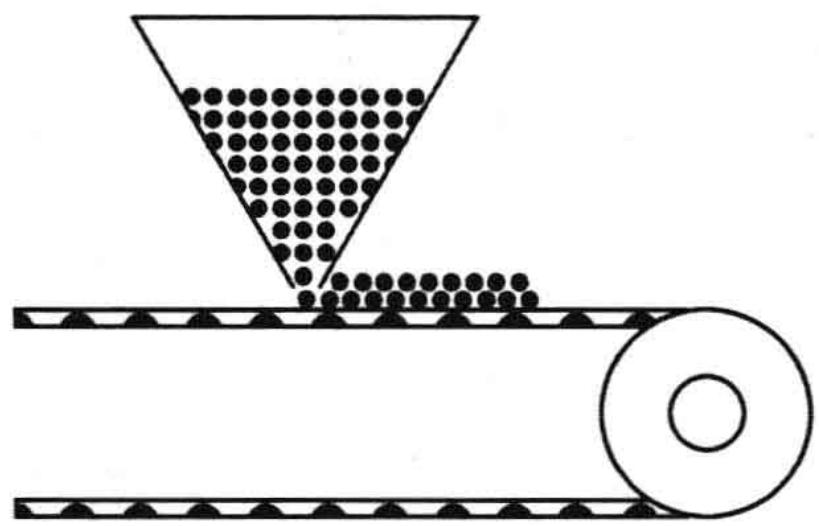
\includegraphics[width=0.25\textwidth]{figures/fig4-23.jpg}
  \end{figure}

\vfill

\textbf{4-24.}一股横截面积为 $S$ 、密度为 $\rho$ 、以绝对速度 $v_{0}$ 在水平方向运动的水流,无弹性地射中一静止在水平面上、质量为 $m$ 的木块,水离开木块时相对于木块的水平速度分量为零。若木块与它在其上滑动的水平面间的摩擦因数为 $\mu$ ,求木块的最终速度。

\vfill
\newpage

\textbf{4-25.}某人用木桶从深井中打水。木桶的质量为 $m_0$ ，刚开始提桶 $(t = 0)$ 时，桶内装有质量为 $m$ 的水，由于桶的底部有一面积为 $S$ 的小洞，桶内的水以相对于桶的恒定速率 $u$ 从洞口流出。

(1) 若人以恒定的速率向上提桶, 求提桶力随时间的变化关系;

(2) 若人以恒力 $F$ 向上提桶, 求水桶在时刻 $t$ 的速率。设 $t = 0$ 时桶静止。

\vfill

\textbf{4-26.}质量为 $m$ 的卡车关闭发动机后在雨中行驶。雨水以速率 $B(\mathrm{kg/s})$ 竖直滴进敞开的车厢内。设 $t = 0$ 时, 车厢是空的, 车速为 $v_{0}$ , 车厢内总共可容纳质量为 $m_{0}(\mathrm{kg})$ 的水。忽略地面对卡车的阻力作用, 试求卡车的速率随时间的变化关系 ( $t$ 从 0 到 $\infty$ )。

\vfill
\newpage

\textbf{4-27.}两质量分别为 $m_{1}$ 和 $m_{2}$ 的小车 A、B 尾尾相接地停在水平路面上, 如习题 4-27 图所示。两车之间用粗绳连接, A 车上装有质量为 $m$ 的水。在 $t = 0$ 时, B 车开始受到一水平恒力 $F$ 的作用, 而 A 车开始以相对于自身的速率 $u$ 把水水平地喷向 B 车, 并全部进入 B 车。设水柱的横截面积为 $S$ , 并忽略地面对两车的阻力作用。试求绳中张力随时间的变化关系。忽略在空中飞行的水柱。

\begin{figure}[H]
  \centering
  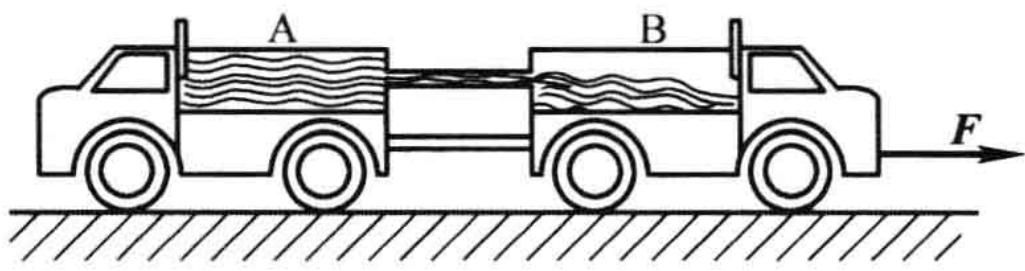
\includegraphics[width=0.4\textwidth]{figures/fig4-27.jpg}
  \end{figure}

\vfill

\textbf{4-28.}若上题中两车之间没有粗绳连接: (1) 在 A 车喷水以后, B 车在外力作用下始终与 A 车保持一定的距离。试求此外力随时间的变化关系; (2) 若两车均无外力作用, 试求在水不能喷入 B 车以前, A、B 两车的速度随时间的变化关系。

以上两小题均忽略地面对车的阻力作用,并可忽略在空中飞行的水柱。

\vfill
\newpage

\textbf{4-29.}如习题 4-29 图所示,一质量为 $m$ 的物体与单位长度的质量为 $\rho_{l}$ 的软绳相连。开始时,物体静置于倾角为 $\theta$ 的光滑斜面的顶端,而软绳则盘放在斜面顶端边的平台上。释放物体,让其沿斜面滑下。求当它下滑距离 x 时的速度。

\begin{figure}[H]
  \centering
  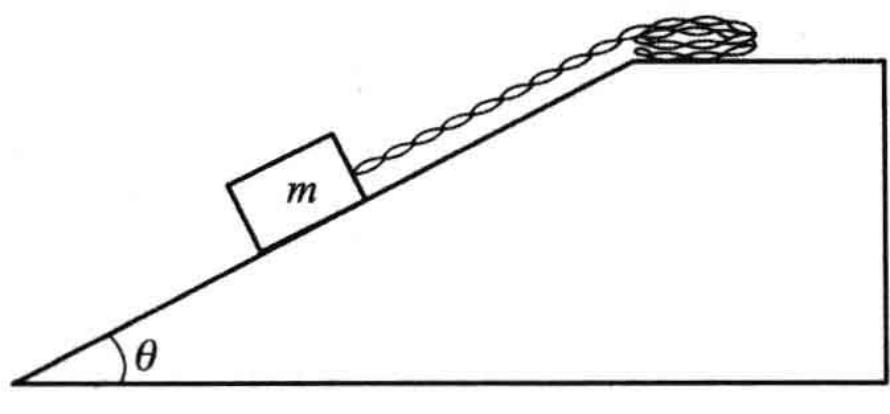
\includegraphics[width=0.3\textwidth]{figures/fig4-29.jpg}
  \end{figure}

\vfill

\textbf{4-30.}线密度为 $\rho_{l}$ 的柔软长链条盘成一团置于地面, 链条的一端系着一质量为 $m$ 的球, 若将球以初速 $v_{0}$ 竖直上抛, 球能上升至多高?

\vfill
\newpage

\textbf{4-31.}从地面发射质量为 $m$ 的火箭（包括燃料），其喷射的燃料气体相对火箭的速度为 $v_{\mathrm{r}}$ ，经过时间 $t_0$ 后，燃料全部喷射完，此时火箭正好获得逃逸速度。设在燃料喷射过程中重力加速度 $g$ 为常量。求空火箭的质量 $m_0$ 。

\vfill

\textbf{4-32.}从地面发射一初始质量为 $m_0$ 的火箭, 喷射的燃料相对火箭的速度为 $v_r$ 。(1) 若其燃料的每秒消耗量 $\frac{\mathrm{dm}}{\mathrm{dt}}$ 可调节, 为使火箭在地面以上某个高度保持静止, 求 $\frac{\mathrm{dm}}{\mathrm{dt}}$ 与时间 $t$ 的函数关系。(2) 若其燃料的每秒消耗量 $\frac{\mathrm{dm}}{\mathrm{dt}}$ 正比于火箭的瞬时质量 $m$ , 即 $\frac{\mathrm{dm}}{\mathrm{dt}} = -\alpha m$ , 其中 $\alpha$ 为正常量。证明当 $\alpha v_r > g$ 时, 火箭将以恒定加速度向上加速, 并求出此加速度。(3) 若其燃料的每秒消耗量 $\frac{\mathrm{dm}}{\mathrm{dt}}$ 正比于 $m_0$ , 即$\frac{\mathrm{d}m}{\mathrm{d}t} = -km_0$ ，其中 $k$ 为正常量。试求火箭在任一时刻 $t$ 的速度。（4）在（3）的情况下，若火箭本身的质量为 $m$ ，试求火箭所能到达的最大高度（不计火箭燃料燃尽后的自由上抛过程）。设火箭到达最大高度时仍未脱离地球引力范围，并设此过程中重力加速度 $g$ 为常量。

\vfill
\newpage

\textbf{4-33.}一火箭总质量为 $m$ , 其中机壳重为 $\beta m$ , 每秒喷出燃料 $\alpha m$ ( $\alpha$ 为常量)。为使火箭在开始喷射燃料的瞬时即能竖直起飞, 燃料的喷射速度 (相对火箭) $v_{r}$ 至少为多大? 维持用这样的速度喷射燃料, 当燃料恰好喷射完时, 火箭上升的最大高度 $h$ 为多少? 设重力加速度 $g$ 为常量。

\vfill
\newpage